\let\negmedspace\undefined
\let\negthickspace\undefined
\documentclass[journal]{IEEEtran}
\usepackage[a5paper, margin=10mm, onecolumn]{geometry}
%\usepackage{lmodern} % Ensure lmodern is loaded for pdflatex
\usepackage{tfrupee} % Include tfrupee package

\setlength{\headheight}{1cm} % Set the height of the header box
\setlength{\headsep}{0mm}     % Set the distance between the header box and the top of the text

\usepackage{gvv-book}
\usepackage{gvv}
\usepackage{cite}
\usepackage{amsmath,amssymb,amsfonts,amsthm}
\usepackage{algorithmic}
\usepackage{graphicx}
\usepackage{textcomp}
\usepackage{xcolor}
\usepackage{txfonts}
\usepackage{listings}
\usepackage{enumitem}
\usepackage{mathtools}
\usepackage{gensymb}
\usepackage{comment}
\usepackage[breaklinks=true]{hyperref}
\usepackage{tkz-euclide} 
\usepackage{listings}
% \usepackage{gvv}                                        
\def\inputGnumericTable{}                                 
\usepackage[latin1]{inputenc}                                
\usepackage{color}                                            
\usepackage{array}                                            
\usepackage{longtable}                                       
\usepackage{calc}                                             
\usepackage{multirow}                                         
\usepackage{hhline}                                           
\usepackage{ifthen}                                           
\usepackage{lscape}
\begin{document}

\bibliographystyle{IEEEtran}
\vspace{3cm}

\title{1-1.6-3}
\author{EE24BTECH11050 - Pothuri Rahul}
% \maketitle
% \newpage
% \bigskip
{\let\newpage\relax\maketitle}

\renewcommand{\thefigure}{\theenumi}
\renewcommand{\thetable}{\theenumi}
\setlength{\intextsep}{10pt} % Space between text and floats


\numberwithin{equation}{enumi}
\numberwithin{figure}{enumi}
\renewcommand{\thetable}{\theenumi}
\textbf{Question}:\\
Determine if the points \brak{1,5} , \brak{2,3} and \brak{-2,-11} are collinear. \\
\solution 
\begin{table}[h!]
    \centering
    \begin{tabular}[12pt]{|c|c|c|}
     \hline
     {parameter} & {discription} & {value}\\
     \hline
     $x_1$ & first intersection point & $\left( \frac{1}{2}, \frac{\sqrt{3}}{2} \right)$ \\
     \hline
     $x_2$ & second intersection point & $\left( \frac{1}{2}, -\frac{\sqrt{3}}{2} \right)$ \\
     \hline
     $V_1$ & \myvec{1-e_1^2 & 0 \\ 0 & 1} & \myvec{1 & 0 \\ 0 & 1}\\
     \hline
     $V_2$ & \myvec{1-e_2^2 & 0 \\ 0 & 1} & \myvec{1 & 0 \\ 0 & 1}\\
     \hline
     $c_1$ & centre of first circle& \myvec{1 \\ 0}\\
     \hline
     $u_1$ & -$c_1$ & \myvec{-1 \\ 0}\\
     \hline
     $c_2$ & centre of second circle& \myvec{0 \\ 0}\\
     \hline
     $u_2$ & -$c_2$ & \myvec{0 \\ 0}\\
     \hline
     $r_1$ & radius of first circle & i \\
     \hline
     $f_1$ & $\lVert u_1 \rVert^2 - r_1^2$ & 0 \\
     \hline
     $r_2$ & radius of second circle & 1\\
     \hline
     $f_2$ & $\lVert u_2 \rVert^2 - r_2^2$ & -1 \\
     \hline 
    $m$ & Slope of the line & \myvec{0 \\ 1}\\
    \hline
    $h$ & Intercept of the line & \myvec{\frac{1}{2} \\ 0} \\
    \hline
    $k_1$ &Parameter of first line & $\frac{\sqrt{3}}{2}$ \\
    \hline
    $k_2$ &Parameter of second line & - $\frac{\sqrt{3}}{2}$ \\
    \hline
     
\end{tabular}
    \caption{Variables Used}
    \label{tab:1.6-3}
\end{table}
\\

The matrix
\begin{align}
\myvec{B-A & C-A}^\top=\myvec{1 & -4 \\ -2 & -14}\\
\xleftrightarrow{R_2 =R_2 +2R_1} 
\myvec{1 & -4 \\ 0 & -22 }
\end{align}
\\
$\therefore$
The rank of matrix is 2. It implies the given points ae non collinear.
\begin{figure}[h]
    \centering
    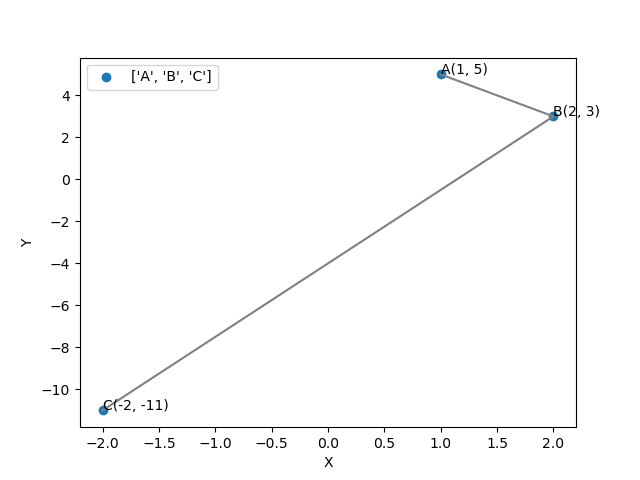
\includegraphics[width=\columnwidth]{figs/fig.png}
    \caption{Plot of A,B,C}
 \end{figure}

\end{document}
